\chapter{系统需求分析}

\section{业务需求概述}
在线个性化学习系统主要服务于学生和教师两大类用户群体。系统的核心业务目标是改变传统 MOOC 平台固定统一化的教学模式，为学习者提供智能导学、交互式知识问答、启发式代码实训以及基于历史行为的个性化课程推荐。教师则通过平台上传视频及文档资源、管理课程、布置作业并监控学生的学习进度。

\section{功能性需求分析}

功能性需求分析主要描述系统应提供的服务声明，即系统应如何对特定输入做出反应以及系统在特定情况下应如何表现。本系统的主要功能涵盖了从用户认证、课程资源浏览、智能AI交互到在线代码实训评测的各个环节。

\subsection{用例图}

以下给出本系统核心模块的用户业务用例图。在用户业务模块中，学生能够进行视频播放、发起智能AI问答、完成代码实训并提交评测，教师能够进行视频上传与习题管理。

\begin{figure}[ht]
  \centering
  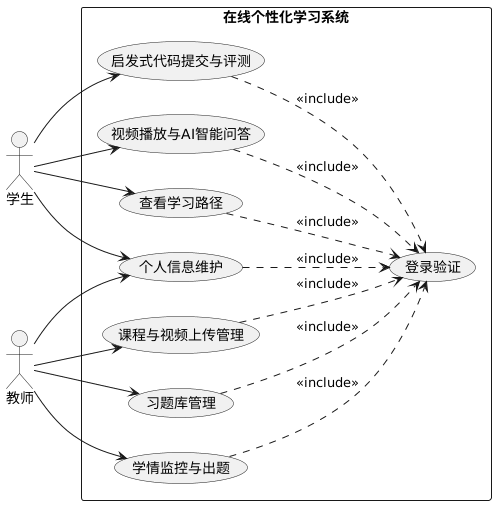
\includegraphics[width=\textwidth,height=0.4\textheight,keepaspectratio]{usecase.png} % 用例图
  \caption{用户业务模块用例图}
  \label{fig:usecase_diagram}
\end{figure}

\subsection{用例规约}

在给出用例图后，以下采用用例规约模板逐个详细描述核心用例。

\vspace{1em}
\noindent\textbf{【用例1：启发式代码提交与评测】}

\noindent\textbf{参与者}：学生（学习者）、评测子系统、大语言模型服务\\
\textbf{目标}：学生希望在不直接获得答案的情况下，通过多次提交代码来获取针对逻辑漏洞或不规范编写的提示，逐步调试并完成题目；系统希望借助AST静态分析和大语言模型的反问式引导，培养学生的独立思考与重构能力。\\
\textbf{包含}：登录验证用例。\\
\textbf{前置条件}：当前学生已登录系统并进入了“智能代码实训与启发调试”页面，且已通过点击获取到了一道对应的Debug或重构实训题。\\
\textbf{触发条件}：学生在代码编辑器中修改代码并点击“提交编译 \& AI评审”按钮。\\
\textbf{主场景}：学生提交代码并获取启发式反馈
\begin{enumerate}
    \item 学生在在线编辑器中编写代码，点击提交按钮。
    \item 前端拦截提交事件，将代码内容、题目信息及当前提交尝试次数打包发往后端API。
    \item 评测子系统接收请求，首先调用Python AST解析器对代码进行静态结构树分析。
    \item 评测子系统生成静态得分及代码缺陷结构报告，将其与预设的苏格拉底系统Prompt结合。
    \item 评测子系统向大语言模型服务发起推理请求。
    \item 大模型服务返回JSON格式的推理结果，包含状态（KEEP\_TRYING或SUCCESS）、启发式反问内容。
    \item 评测子系统校验结果无误后将其返回给前端。
    \item 前端解析并渲染AI反馈内容，同时更新左侧界面的当前尝试次数和状态徽章。
\end{enumerate}
\textbf{主场景后置条件}：
\begin{enumerate}
    \item 学生的本次提交记录（包含代码原文、尝试次数、大模型反馈、静态得分）成功保存至数据库。
    \item 学生界面能够正确且清晰地展示出AI教师的苏格拉底式评语，并未泄露最终正确代码。
\end{enumerate}
\textbf{其他场景}：达到最大尝试次数限制
\begin{enumerate}
    \item 学生提交代码后，后端检测到尝试次数已达上限（如5次）。
    \item 评测子系统更改大模型调用的指令，允许其输出包含最终正确代码的解析。
    \item 大模型返回状态为 MAX\_TRIES\_REACHED，并附带了最终参考答案。
    \item 前端渲染红色状态警告，并展开显示正确参考代码。
\end{enumerate}
后置条件：系统锁定该题目的后续启发式提交尝试，并开放答案供学生直接比对学习。\\
\textbf{异常场景}：等待大语言模型服务响应超时
\begin{enumerate}
    \item 评测子系统向大语言模型发起请求。
    \item 网络延迟或模型服务拥塞，超过5秒未返回结果。
    \item 后端自动熔断，向前端返回“AI评审服务当前繁忙，请稍后重试”的错误状态。
\end{enumerate}
后置条件：学生的尝试次数不计增加，前端给出网络异常的弱提示。\\
\textbf{发生频率}：高峰期可能达到每分钟数十次并发提交。\\
\textbf{限制}：评测系统沙箱必须完全屏蔽 \texttt{os}、\texttt{sys} 等系统级别危险调用。

\vspace{1.5em}
\noindent\textbf{【用例2：视频播放与AI智能问答】}

\noindent\textbf{参与者}：学生、文档/向量检索服务、大语言模型服务\\
\textbf{目标}：学生在观看课程视频遇到不懂的概念时，可以向右侧的AI助手提问，AI助手能够结合当前视频的上下文给出解释，并给出可点击跳转的引用来源。\\
\textbf{前置条件}：当前学生处于课程视频播放页面。\\
\textbf{触发条件}：学生在AI助手对话框中输入问题并按下回车键。\\
\textbf{主场景}：学生提问获取带有溯源角标的回答
\begin{enumerate}
    \item 学生在对话框输入问题，如“这里讲的线性回归算法原理是什么？”
    \item 前端将问题内容及当前页面的 \texttt{videoId} 发送至流式问答API。
    \item 文档/向量检索服务利用 FAISS 索引查询该视频对应的字幕文本片段。
    \item 后端聚合检索结果构建Prompt，提交给大模型。
    \item 大模型流式返回包含引用标记（如 \texttt{[1]}）的 Markdown 文本。
    \item 前端解析 Markdown，将引用标记渲染为可点击交互的组件。
\end{enumerate}
\textbf{主场景后置条件}：
\begin{enumerate}
    \item 对话界面完整展示解答与引用角标。
    \item 会话消息持久化存入数据库。
\end{enumerate}
\textbf{其他场景}：点击角标跳转
\begin{enumerate}
    \item 学生点击回复文本中的引用角标 \texttt{[1]}。
    \item 前端事件委托机制捕获点击，读取绑定的视频时间点。
    \item 视频播放器自动 Seek 跃迁至该时间点并开始播放。
\end{enumerate}

\section{非功能性需求分析}

非功能性需求定义了整个系统的质量特性，确保系统在高效、安全、可靠的环境下运行。

（1）\textbf{性能需求}：
\textbf{响应速度}要求单页面加载（如获取学习任务、浏览视频列表）时间不得超过 3 秒。大语言模型流式问答的首次响应延迟（Time To First Token, TTFT）需低于 2 秒，以保证对话的流畅性。
\textbf{并发处理能力}要求在并发访问高峰期（例如100个用户同时进行在线代码提交与AI交互），后端的 Flask 框架及 Gunicorn 服务器应能稳定处理，代码隔离沙箱运行单个脚本的耗时必须限制在 5 秒以内，以防资源耗尽。系统吞吐量 $TPS = \frac{N}{T}$ 需满足设计预期指标。

（2）\textbf{可靠性需求}：
\textbf{容错性}方面，对于视频转码或文档向量化等长耗时异步任务，必须具备失败重试与死信队列机制。如果 ASR 语音识别失败，任务不应导致主服务崩溃，而应将记录标记为失败状态并通知管理员。
\textbf{数据一致性}方面，大语言模型问答过程中，如果用户主动关闭浏览器中断连接，服务端应能正确捕获中断信号，中止流生成并进行数据库的清理与消息持久化封装。

（3）\textbf{安全需求}：
\textbf{身份认证与权限管控}方面，平台接口必须采用 JWT（JSON Web Token）或同级别的无状态鉴权机制，只有携带有效 Token 的请求才能访问敏感数据及调用大模型接口。
\textbf{代码执行安全}方面，在智能实训模块中，使用动态执行代码环境（如 \texttt{exec}）时，必须置入只读沙盒（Sandbox）环境，屏蔽任何 I/O 写操作或系统级调用。
\textbf{隐私保护}方面，用户的注册密码必须采用强哈希算法（如 bcrypt）加盐存储，防止数据库泄露导致密码明文暴露\cite{whu-bachelor:26}。

（4）\textbf{可用性与易用性需求}：
\textbf{跨端支持}方面，前端界面应当支持响应式布局（Responsive Design），适配 PC 端浏览器及一定程度的平板浏览器视图。
\textbf{操作提示}方面，所有的功能点应当具备清晰友好的交互反馈。例如，长耗时的代码验证期间，需在按钮处展示明显的 Loading 状态并禁用按钮，防止用户的重复恶意点击。

\section{约束}
本系统的开发与运行受到以下约束：

\textbf{项目约束}：开发周期限制为毕业设计规定时间内（约4个月）完成，故大语言模型服务直接调用成熟的云端 API（如文心一言或智谱等）而不在本地进行预训练，仅在本地运行向量数据库。

\textbf{物理约束}：服务器硬件资源有限（4核 8G 内存），因此所有的文本向量化和密集型计算任务必须合理控制进程数量，以避免发生 OOM（Out Of Memory）错误。内存使用量 $M$ 需满足 $M_{req} \le M_{max} \times 80\%$ 的安全阈值。

\textbf{技术约束}：前端限定采用 Vue 3 生态，以确保符合现代 Web 工程化的要求；后端限定采用 Python 技术栈，以便无缝集成各项 AI 和自然语言处理相关的 SDK 工具包。
